\documentclass{article}
\usepackage[english]{babel}
\usepackage{verbatim}
\usepackage{graphicx}
\usepackage{url}
\usepackage{float}
\title{Knowledge Based Systems Solution Search A1}
\author{Laura Khaze \& Erik Zeiske}
\date{10 April 2019}
\makeatletter
\newcommand{\problem}{Schatzsuche - das dreiteilige Medaillon}
\begin{document}
\begin{titlepage}
    \begin{center}
        \vspace*{1cm}
 
        \Huge
        \textbf{\@title}
 
        \vspace{0.5cm}
        \LARGE
        A documentation outlining the implementation of the problem \textit{\problem}
 
        \vspace{1.5cm}
 
        \textbf{\@author}
 
        \vfill
        INF 16A\\
        DHBW Stuttgart\\
        \@date
       
        \vspace{1.8cm}
 
        %\Large
        Knowledge-based Systems \\
        Prof. Dr. Dirk Reichardt \\
        Applied Computer Science
 
 
    \end{center}
\end{titlepage}
%\tableofcontents
%\newpage
\section{Problem Formulation} \label{problem_formulation}
The goal of the game \textit{\problem} is to compose a locket. The locket consists of three different components of type A, B and C. To compose the locket a player needs one component of each type. \\
The components of the locket are spread over the playground which consists of three different lands and some water areas. Within the playground a player can move either left, right, up or down as long as he does not enter a water area or leave the playground. Moreover it is not possible for the player to cross the border between land L1 and L2 if a component of type B is in his possession. \\
To solve the given problem, find all components and win the game the $A^*$ algorithm is implemented. \\

\section{Definitions}
In the following some terminologies are defined to create a common basis for this documentation.
\begin{description}
    \item{\textbf{Player}} The individual that moves around in order to find all components of the locket (For visual speaking purposes)
    \item{\textbf{Land}} There are three different lands. A land is either of type L1, L2 or L3.
    \item{\textbf{Field}} A field is described by an x y position whereby x describes the horizontal position while y states the vertical position. It is part of exactly one land or is water. It can either be empty or contain exactly one component.
    \item{\textbf{Playground}} All fields arranged in a $m x n$ grid whereby m is the height and n is the width of the playground (start counting at 0).
    \item{\textbf{Components}} A component is either of type A,B or C. At least one copy ($n \geq \ $1) of each type is laying scattered on one field of the playground.
    \item{\textbf{State}\label{definition_state}}  Is a node of the graph to traverse with $A^*$ and is uniquely defined by the x and y position on the field and which components are already collected. 
    This means that a state can be represented as $S(x,y,A,B,C)$ where $x$, $y$ state the x and y coordinates of the associated field the player is currently on and $A, B, C$ weather he is holding the respective components. If a variable x,y or A, B, C is notated within a state this means the value in this field can be anything.\\
    Thus $S(2,1,0,0,1)$ is the state on which the player is on field $(2,1)$ and holds only the component of Type C.
    \item\textbf{ Distance function $k(S_1, S_2)$} This function is used to determine the shortest distance between two fields.
    \item \textbf{Estimation function {$h(S)$}} This function is used to estimate the shortest distance to any termination state.
    \item \textbf{Cost function {$h^*(S)$}} This function determines the actuall shortest distance to any termination state.
\end{description}

\section{Assumptions}
In order to implement a solution to the given problem \textit{\problem} it is necessary to make some assumptions about the details of the problem formulation. These assumption are:
\begin{enumerate}
    \item It is possible for a player to move through a field without picking up the component it is holding. 
    \item When a component was picked up it can not be laid down again.
    \item Since there is no added value it is not possible for a player to possess two components of the same type.
\end{enumerate}


\section{$A^*$ Algorithm}
To solve the problem formulation given in \ref{problem_formulation} with the $A^*$ algorithm the following points are decided and documented.
\begin{comment}
\begin{itemize}
    \item Development of an graph
        \begin{itemize}
            \item What state does a node describe
            \item Set of terminating nodes
        \end{itemize}
    \item Distance function for the graph $k(S_1, S_2)$
    \item Estimation function $h(S)$
\end{itemize}
\end{comment}

\subsection{Graph Definition}
In order to define a graph first of all a node (i.e. a state) has to be defined: As the player can only be distinctly on a field it is only logical to associate the state to a field and a transition between the states to the movement between two fields. Also the players state should contain which components he has collected yet. See section \ref{definition_state} for an exact definition. As the player can move only right, left, up and down the possible changes from a movement point of view are:
% TODO add picture with x,y as coordinates and x+-1 / y+-1 respectively.
These movements might be blocked if the neighboring field is out site of the playground, the destination field is water or the player tries to cross the border between L1 and L2 (both directions).
\subsection{Distance function  $k(S_1, S_2)$}
Since a move between two fields takes one minute every movement state transition is associated with $k(S_1, S_2) = 1$.\\
As there is no downside to automatically picking up the component A and C, every move to a field containing one of these components will move the player to a state where the respective component is in their possession. In case of a field containing B the move to this field will not automatically pick up the component as it might block movement later on. Thus it is possible to explicitly pick up the component on such a field with no cost to the movement ($k(S(x,y,A,0,C), S(x,y,A,1,C)) = 0$).\\
All states of the form $S(x,y,1,1,1)$ are terminating states.

\subsection{Estimation function $h(S)$}
The goal of the implementation is to collect all components. Thus the shortest and best possibility to do so, is to go through all missing components taking the shortest path between them. \\
The shortest distance between two nodes can be determined by the Manhattan distance as the player can only move horizontally and vertically (without consideration of blocked movement due two water or the borders between two lands). Since the distance function equals one for each movement between two nodes ($k(S_1, S_2) = 1$) the Manhattan distance can be used as $h(S)$ to estimate the path between two components.
This way an optimistic $A^*$ algorithm is ensured, since $h(S) \geq \ h^*(S)$.

 For example if the player is already holding A and B the estimation has to take the Manhattan distance to all C components and return the minimum of these distances. Respectfully if no components are held by the player all possible orders of going through the components have to be associated with there respective distances and the shortest is the estimate for the state. As the distance between the components is not changing the estimation from the component fields can be cached, see section \ref{estimation_caching_tables}. %TODO add reference


\section{Implementation}
The implementation of the $A^*$ algorithm is realized in C++ and was written on a windows system using msys2 (\url{https://www.msys2.org/}).
\subsection{Input and Output}
The implementation requires six inputs and returns the best route as an output.\\
Example input: \textit{20 20 "data/spielfeld\_1.csv" "data/S11.txt" 0 0 color}\\
%Example output: \textit{(0,0) - (0,1)}
\begin{description}
    \item{\textbf{Input playground size}} The first two input parameters \textit{m n} define the size of the playground $m x n$ whereby m is the height and n is the width of the playground. %grid width, height
    \item{\textbf{Input playground}} The third input parameter is a csv file with the playground itself. Thereby each land type is represented by one number: L1 is represented by a 1, L2 by 2, L3 by 3 and water by 0. If the given playground is bigger than the size given by the parameters \textit{m n} a playground of size \textit{m n} is realized.
    \item{\textbf{Input components}} The fourth input parameter is a text file which contains the coordinates of the components in the format \textit{Type;X;Y}.
    \item{\textbf{Input start position player}} The fifth (x) and sixth (y) parameter set the start coordinates (x,y) of the player.  If the start position of the player is outside of the playground or on a water field an error message is thrown.
    \item{\textbf{Input Color}} This parameter can be used to request a colored output. If this parameter is not set the output is plain.
    \item{\textbf{Output route}} The program returns the best route as an output. The single state $S(x,y,A,B,C)$, in the format \textit{(x, y)CBA g=p h=q}), of the route are printed in the reverse order.
\end{description}

\subsection{Program Structure}
Since the source code of the program is well annotated only some main ideas and strategies are explained in this section.\\
The $A^*$ algorithm is implemented with four different classes: Component, Playground, PriorityQueue and State as well as the namespace helper. 

\begin{description}
    \item[Component] Every instance of this class has a type (A, B or C) saved as bits. A is represented by 001, B by 010 and C by 100. Due to the bit representation it is possible to use a bit mask and use different bit shifting operations. Moreover a caching table is saved within this class, see \textit{\ref{estimation_caching_tables} Estimation Caching Tables}.
    \item[Playground] This is the main class holding all required objects. It has a list of all components which is used for the estimation calculation. Moreover an array with a bitmask for every field is saved within this class.
    \item[PriorityQueue] This is the class designed to store the openList for the $A^*$ algorithm. It is possible to store states in a priority queue whereby the state with the smallest sum of g and h is returned by the \textit{pop} function. As the source code is written in C++ it was necessary to implement a own priority queue to update the priority (g + h) later on to avoid constant adding and removing to the priority queue. Since it is not necessary to have a sorted list, a heap is used to implement the priority queue. 
    %As the source code is written in C++ (memory management) a priority queue which enables the user to update the weight g of the elements later on and rearranges the elements accordingly is preferred. Due to the required functionalities a generic priority queue was not used.
    \item[State] This class realises the given definition of a state ($S(x,y,A,B,C)$). It stores the x and y coordinates as well as whether or not a component i in the possession of the player. Furthermore the values g and h are stored within the state, whereby g is the shortest known path to the state and h is the estimated distance to a final state ($S(x,y,1,1,1)$).
    \item[Helper] In this namespace some helper functions which do not belong to one specific class are implemented.
\end{description}
\begin{comment}
\subsection{Klassen}
Artifact

playground
erzeugt durch einlesen der files, basic object
calculate path --> hauptfunction
getEstimate, unser H
bitmaske artifact
artifact, bitmaske 
\end{comment}


\subsection{Estimation Caching tables} \label{estimation_caching_tables}
Each instance of the class component saves its own caching table. In this table the estimated distance from the specific component to collect all other components is saved. This example is a caching table of a component A:\\
\begin{center}
\begin{tabular}{ |c|c|c|c|c|c| } 
 \hline
 %\multicolumn{3}{|c|}{CBA}
 C & B & A & $h(S)$ & level \\ 
 \hline
 0 & 0 & 0 & 13 & 0 \\ 
 0 & 0 & 1 & 13 & 0 \\ 
 0 & 1 & 0 & 5 & 1 \\ 
 0 & 1 & 1 & 5 & 1 \\ 
 1 & 0 & 0 & 9 & 1 \\ 
 1 & 0 & 1 & 9 & 1 \\ 
 1 & 1 & 0 & 0 & 2 \\ 
 1 & 1 & 1 & 0 & 2 \\ 
 \hline
\end{tabular}
%\caption{Caching table of a component A}
\label{tab:caching table}
\end{center}
If the component is already in the possession of the player when he enters the field a 1 is saved in the table otherwise a 0. 
The caching table is filled and saved within the component since, due to the assumption 2, the table will not change. 
The level is the number of components which are already in the possession of the player, not counting the type of the component the table is saved in. 
Since the Manhattan distance is used as an optimistic estimation function the triangle equation is true. This enables the calculation of $h(S)$ based on the $h(S)$ value of the next higher level.


\section{Testing}
In order to test the implementation of the \textit{\problem} several tests were designed and performed. The test were performed ten times each to ensure the implementation is deterministic. 

\subsection{Test 1}
The program is tested on a given playground ($20 x 20$, \textit{spielfeld\_1.csv}) with a given distribution of components (\textit{S11.txt}).\\
%(5,3)->L1, (15,15)->L3 and (13,19)->water.\\
\textbf{Playground}:\\
\begin{figure}[H]
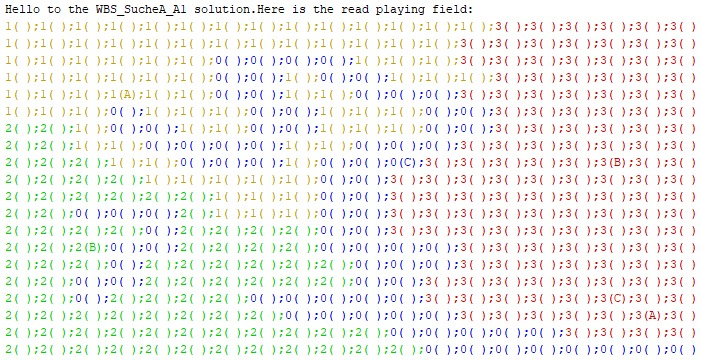
\includegraphics[width=14cm]{playgroundtest1.jpeg}
\centering
\end{figure}

\subsubsection*{Test 1 - start position (5,3)}
The player starts on a flied of type L1 and is able to find all components. The program determines a route and prints the output in a reserve order. \\
\textbf{Input}:\\
\texttt{WBS\_SucheA\_A1.exe 20 20 data/Testing/test1.csv data/Testing/test1.txt 5 3 color}\\
\textbf{Output}:
\begin{figure}[H]
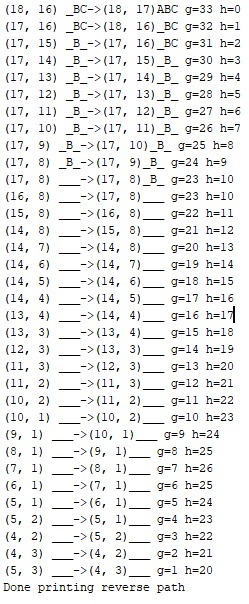
\includegraphics[width=6cm]{start53}
\centering
\end{figure}

\subsubsection*{Test 1 - start position (15, 15)}
The player starts on a flied of type L3 and is able to find all components. The program determines a route and prints the output in a reserve order. \\
\textbf{Input}:\\
\texttt{WBS\_SucheA\_A1.exe 20 20 data/Testing/test1.csv data/Testing/test1.txt 15 15 color}\\
\textbf{Output}:
\begin{figure}[H]
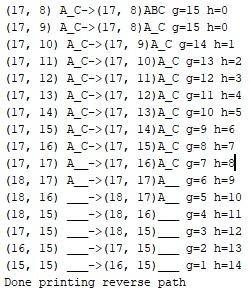
\includegraphics[width=6cm]{start1515}
\centering
\end{figure}

\subsubsection*{Test 1 - start position (13,19)}
The player starts on a water field and is not able to find all components, since it is not possible. The program terminates. \\
\textbf{Input}:\\
\texttt{WBS\_SucheA\_A1.exe 20 20 data/Testing/test1.csv data/Testing/test1.txt 15 15 color}\\
\textbf{Output}:
\begin{figure}[H]
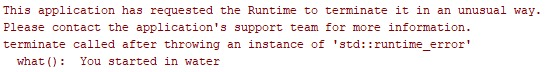
\includegraphics[width=14cm]{waterstart}
\centering
\end{figure}

\subsection{Test 2}
A one dimensional playground ($1 x 7$) where the player starts on (0,0) and has to cross the border between L1 and L2 without the component B in order to compose the locket:\\ 
\begin{comment}
\textbf{Playground ($1 x 7$)}

\begin{tabular}{ |c|c|c|c|c|c|c|c|c| } 
 \hline
 & 0 & 1 & 2 & 3 & 4 & 5 & 6 \\ 
 \hline
 0 & L1 & L1 & L1 & L2 & L3 & L2 & L3 \\ 
 \hline
\end{tabular}
\\


\textbf{Components}

\begin{tabular}{ |c|c|c| } 
 \hline
 x & y & type  \\ 
 \hline
 0 & 1 & A \\
 0 & 2 & B \\
 0 & 6 & C \\ 
 \hline
\end{tabular}
\end{comment}
\\
\textbf{Input}:\\
\texttt{WBS\_SucheA\_A1.exe 1 7 data/Testing/test2.csv data/Testing/test2.txt 0 0 color}\\
\textbf{Output}:
\begin{figure}[H]
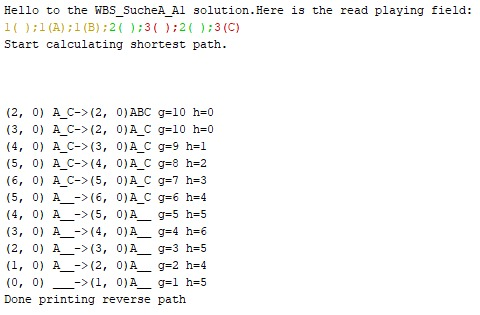
\includegraphics[width=14cm]{test2}
\centering
\end{figure}

\subsection{Test 3}
A  playground ($5 x 5$) where the player starts on an island (2,2) and there is no possible way to collect all components.
\begin{comment}
\textbf{Playground ($5 x 5$)}

\begin{tabular}{ |c|c|c|c|c|c|c| } 
 \hline
 & 0 & 1 & 2 & 3 & 4  \\ 
 \hline
 0 & L1 & L1 & L1 & L2 & L3 \\ 
 \hline
 1 & L1 & W & W & W & L3 \\ 
 \hline
 2 & L1 & W & L1 & W & L3 \\ 
 \hline
 3 & L1 & W & W & W & L3 \\ 
 \hline
 4 & L1 & L1 & L1 & L2 & L3 \\ 
 \hline
\end{tabular}
\\
\textbf{Components}

\begin{tabular}{ |c|c|c| } 
 \hline
 x & y & type  \\ 
 \hline
 0 & 1 & A \\
 0 & 2 & B \\
 4 & 4 & C \\
 3 & 4 & C \\ 
 \hline
\end{tabular}
\end{comment}
\\
\\
\textbf{Input}:\\
\texttt{WBS\_SucheA\_A1.exe 5 5 data/Testing/test3.csv data/Testing/test3.txt 2 2 color}\\
\textbf{Output}:
%\end{comment}
\begin{figure}[H]
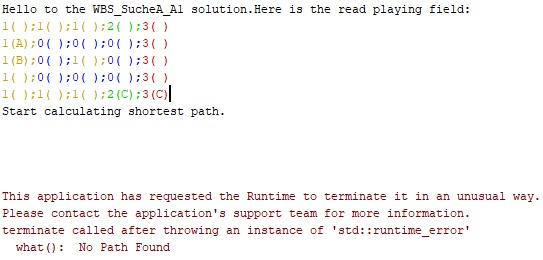
\includegraphics[width=14cm]{test3}
\centering
\end{figure}


\section{Evaluation and possible Improvement}
It is possible to find a shorter and thereby better way to collect all components and thus win the game if assumption 2 would be disregarded. 
This would increase the expenditure of the implementation tremendously since for example it would prohibit the usage of estimation caching tables as explained in subsection \ref{estimation_caching_tables}. This is one possible improvement for the future.\\
%One lesson learned for the future is the choice of C++ as a programming language. 
%On the end of the implementation it was noticed, that some used c++ features (generating varying size arrays based on runtime variables) is not implemented in the visual studio compiler. Thus it was not possible to generate a executable directly for native windows.

\end{document}